\documentclass{beamer}

\usecolortheme[light]{solarized}

\beamertemplatenavigationsymbolsempty

\usepackage{hyperref}

\usepackage{booktabs}
\usepackage{graphicx}
\usepackage{minted}
\usepackage{moresize}
\usepackage{standalone}
\usepackage{tcolorbox}
\usepackage{tikz}
\usepackage[normalem]{ulem}
\usepackage{xpatch}

\xpatchcmd{\sout}
  {\bgroup}
    {\bgroup\def\ULthickness{2pt}}
      {}{}

\usetikzlibrary{calc, patterns}

\definecolor{twitter}{RGB}{64, 153, 255}
\definecolor{github}{RGB}{211, 211, 211}

%\newcommand{\assetsfolder}{../2017-08-31-Handshakes-citizen-science-and-evolution/assets}
%\newcommand{\researchfolder}{$HOME/rsc/axelrod-moran}
%\newcommand{\mlresearchfolder}{$HOME/rsc/ml-paper}

\begin{document}

    \begin{frame}
        \begin{center}
            \Large
               Vince: \href{https://twitter.com/drvinceknight}{@drvinceknight}\\
        \end{center}
    \end{frame}

    \begin{frame}
        \begin{center}
            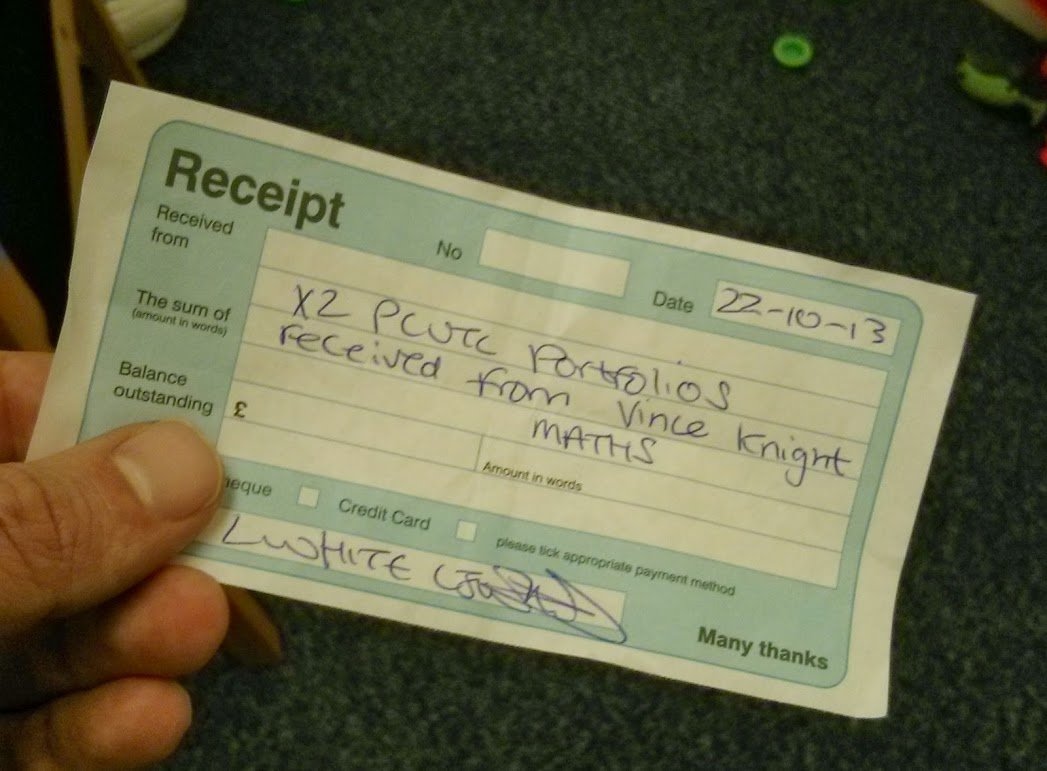
\includegraphics[width=.8\textwidth]{../2015-07-22-My-experience-of-pcutl/pcutl.jpg}
        \end{center}
    \end{frame}

    \begin{frame}
        \begin{center}
            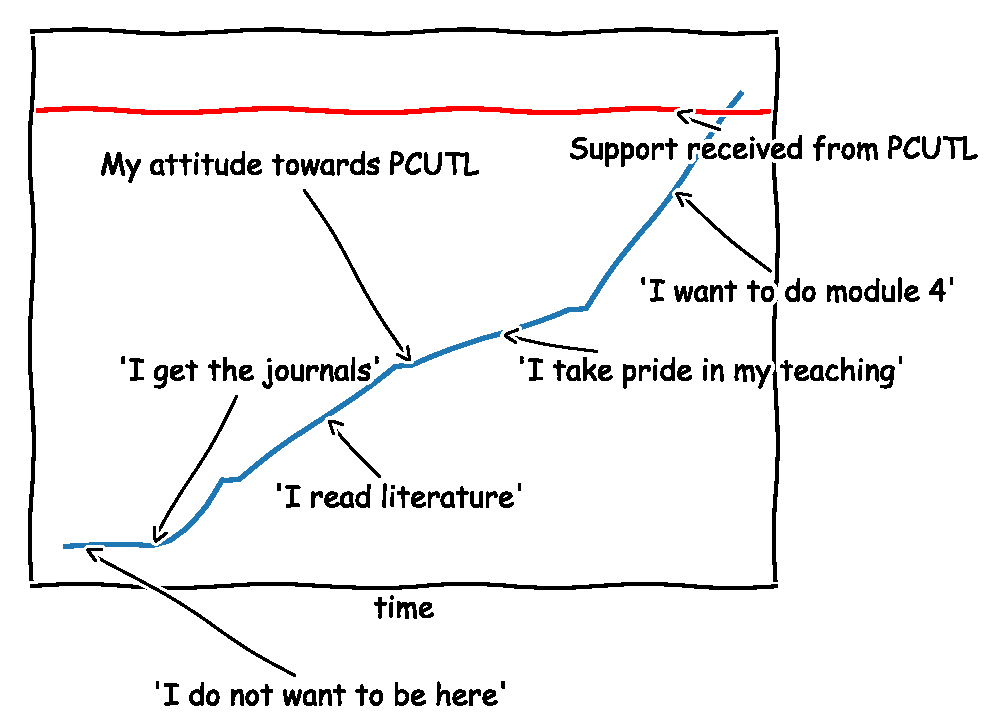
\includegraphics[width=.8\textwidth]{./assets/xkcd_pcutl.pdf}
        \end{center}
    \end{frame}

    \begin{frame}
        \begin{center}
            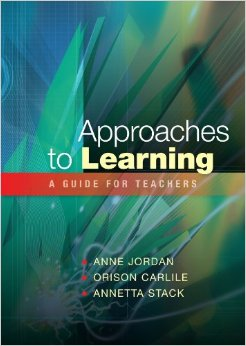
\includegraphics[height=.8\textheight]{../2015-07-22-My-experience-of-pcutl/approaches_to_learning.jpg}
        \end{center}
    \end{frame}

    \begin{frame}
        \textbf{Lecture}

        \begin{quote}
            An educational talk to an audience, especially one of students in a university.
        \end{quote}
    \end{frame}

    \begin{frame}
        \textbf{Lecture}

        \begin{quote}
            A long serious speech, especially one given as a scolding or reprimand.
        \end{quote}
    \end{frame}


    \begin{frame}
        \textbf{Lecture}

        \begin{quote}
           Deliver an educational lecture or lectures.
        \end{quote}
    \end{frame}

    \begin{frame}
        \textbf{Lecture}

        \begin{quote}
            Talk seriously or reprovingly to (someone).
        \end{quote}
    \end{frame}

    \begin{frame}
            Bligh 1972: What's the Use of Lectures?
    \end{frame}

    \begin{frame}
        \begin{center}
            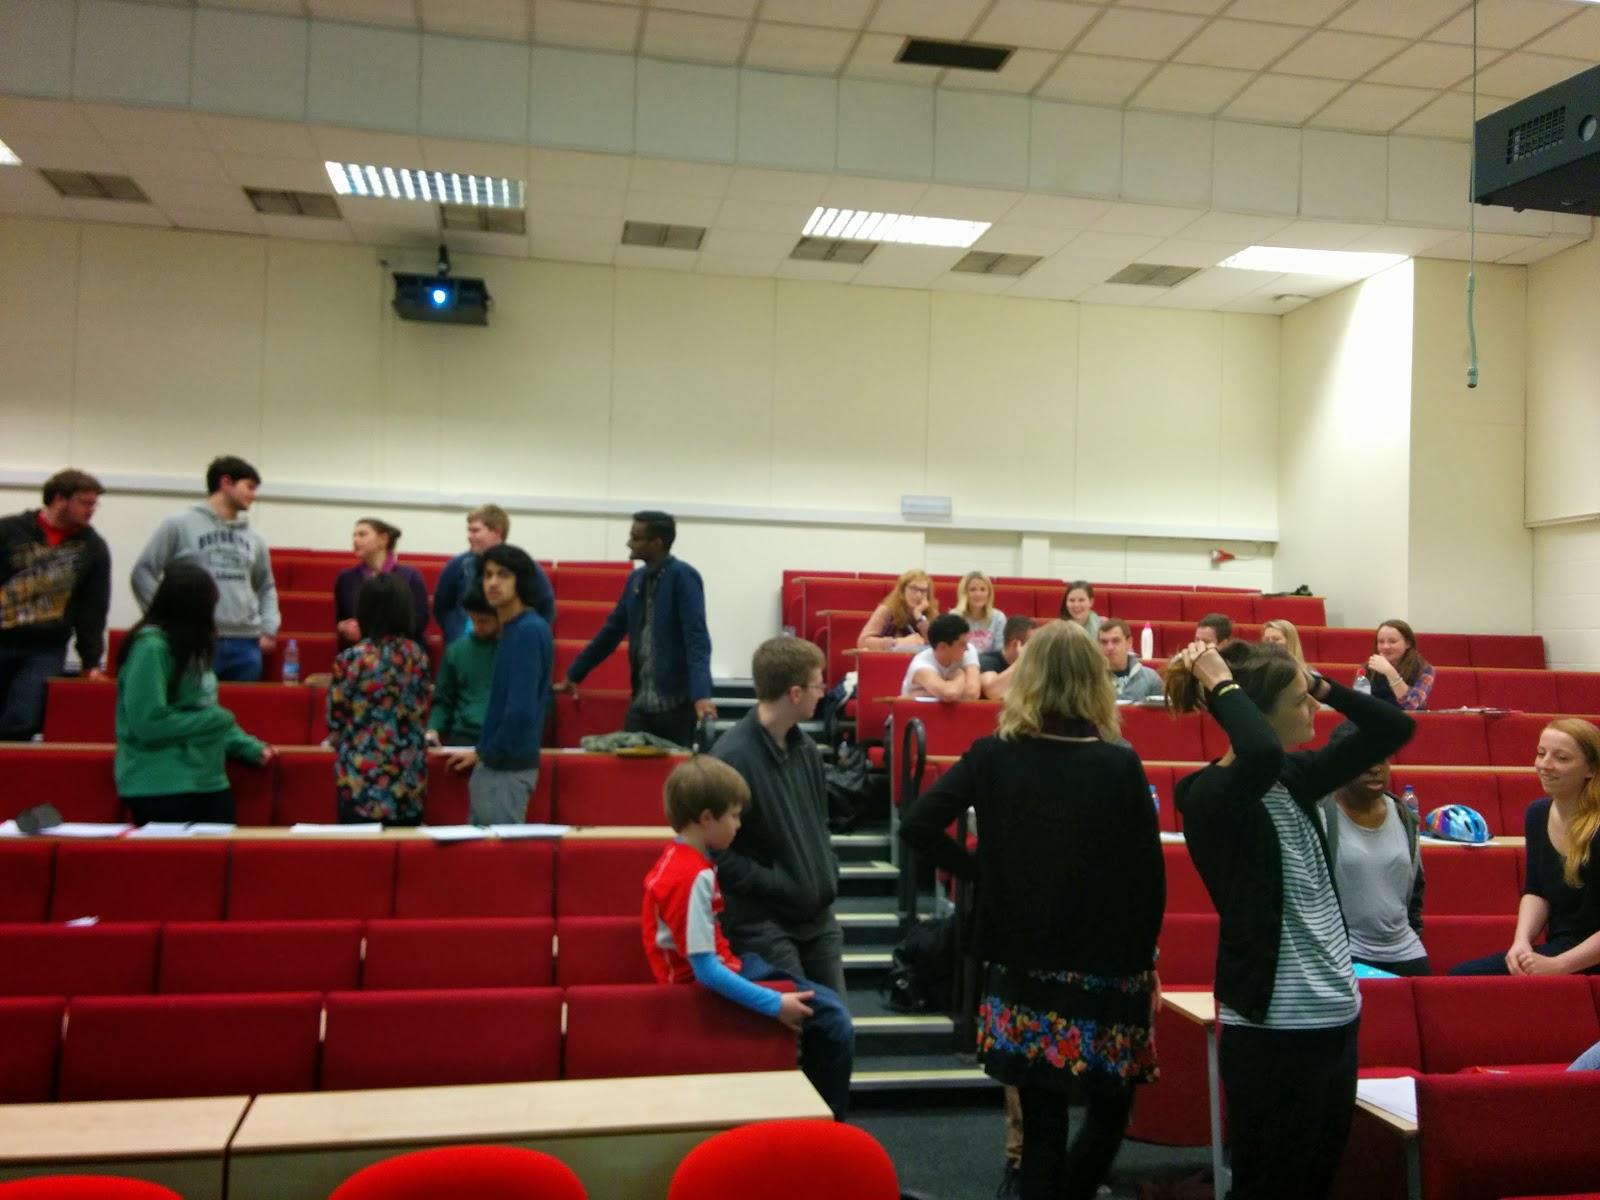
\includegraphics[width=.8\textwidth]{../2016-07-07-What-is-the-lecture-for/img/class_meeting.jpg}
        \end{center}
    \end{frame}

    \begin{frame}
        \begin{center}
            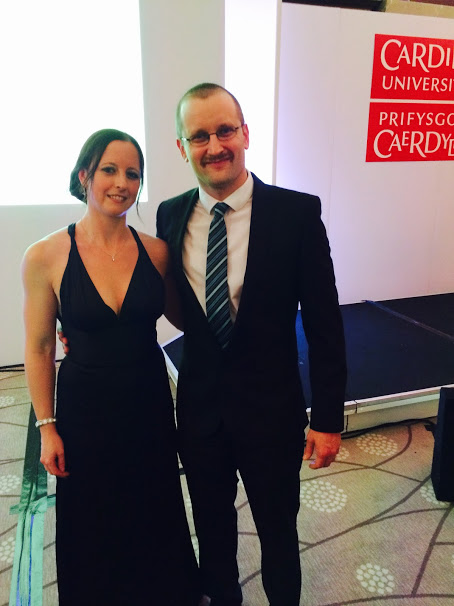
\includegraphics[height=.8\textheight]{../2015-07-22-My-experience-of-pcutl/prize.jpg}
        \end{center}
    \end{frame}
\end{document}
